\documentclass[11pt]{article}

\usepackage{amsmath,amssymb,amsfonts}
\usepackage{graphicx}
\usepackage{pgfplots}
\usepackage{multicol}
\usepackage{enumitem}
\usepgfplotslibrary{fillbetween}
\pgfplotsset{compat=1.16,width=10cm}


\setlength{\topmargin}{-.5in} \setlength{\textheight}{9.25in}
\setlength{\oddsidemargin}{0in} \setlength{\textwidth}{6.8in}


\begin{document}

\Large

\noindent{\bf Name: \hfill Date: \hfill Exam 3 \hfill AP Calculus - Hargus}

\medskip\hrule
\vspace{10pt}

\noindent \textbf{Instructions:} Please \textbf{show all work} on the test paper (partial credit may be awarded for correct work, even if your answer is wrong). You may use the back side if you run out of room. Calculators are not allowed, but \textbf{simplify} your answers as much as you can. Cheating of any kind will result in a score of zero.

\vspace{10pt}

\begin{enumerate}[itemsep=30pt]

\item (8 points) Label \textbf{all} points of inflection, local minimums, and local maximums. Then, between each of these transition points, label the graph with the sign of $f'(x)$ and $f''(x)$. For example, if $f'(x)>0$ and $f''(x)<0$ for some part of the graph, then write $+-$ next to that part of the graph.
\vspace{10pt}
\begin{center}
\begin{tikzpicture}
\begin{axis}[ xlabel={$x$}, ylabel={$y$}
  ,axis lines=middle
  ,height=7cm
  ,width=12.5cm
  ,samples=1000, grid, thick
  ,domain=-10:10
  ,restrict y to domain=-10:10
  ,axis equal
  ,legend pos=outer north east
  ,xmin=-2, xmax=5,
  ,ymin=-2, ymax=2.5
  ];
\addplot+[no marks] {sin(x*180/pi)+x/2};
\end{axis}
\end{tikzpicture}
\end{center}


\item (4 points) If $\lim_{x \to 1} f(x) = \infty$, what kind of asymptote does $f(x)$ definitely have (circle your answer: \textbf{horizontal} or \textbf{vertical}) and what is the equation for that asymptote's line?
\begin{flushright}
Equation for asymptote: \rule{4cm}{0.4pt}
\end{flushright}

\newpage


\item (12 points) Find the derivative $f'(x)$:
\begin{enumerate}[itemsep=40pt]
    \item{$f(x) = x^4 + x^2$}
    \item{$f(x) = x^{\frac{1}{3}}$}
    \item{$f(x) = (2x + 3)^4$}
    \item{$f(x) = 4^x$}
    \item{$f(x) = x \sin(x)$}
    \item{$f(x) = \sec(x)$}
\end{enumerate}

\vspace{20pt}
\item (4 points) Find the \textbf{second derivative} $y''$ for the given $y$:

\begin{enumerate}[itemsep=80pt]
    \item{$y = -x^2 + 2x^3$}
    \item{$y = 8x^{\frac{1}{2}}$}
\end{enumerate}



\newpage

\item (8 points) Evaluate the limit:
\begin{multicols}{2}
\begin{enumerate}[itemsep=80pt]
    \item $\displaystyle{\lim_{x \to 77} 5}$
    \item $\displaystyle{\lim_{x \to \infty} \frac{5x^{10}}{x^{10} + 3}}$
    \item $\displaystyle \lim_{x \to 1} \frac{3x^3 - 3}{2-3x^2 + x} $
    \item $\displaystyle \lim_{x \to \infty} \frac{e^x}{x} $
\end{enumerate}
\end{multicols}

\vspace{50pt}


\item (4 points) For the graph below, draw the derivative function $f'(x)$ on the same graph below (does not need to be exact, though x-intercepts and sign ($+$/$-$) should be correct):

\vspace{10pt}
\begin{center}
\begin{tikzpicture}
\begin{axis}[ xlabel={$x$}, ylabel={$y$}
  ,axis lines=middle
  ,height=10cm
  ,width=10cm
  ,samples=1000, grid, thick
  ,domain=-10:10
  ,restrict y to domain=-10:10
  ,axis equal
  ,legend pos=outer north east
  ,xmin=-3, xmax=4,
  ,ymin=-2, ymax=2
  ]
\addplot+[no marks] {-(x-3)*(x+1)*(x+1)/5};
\addlegendentry{$f(x)$}
\end{axis}
\end{tikzpicture}
\end{center}

\newpage

\item (12 points) Evaluate the indefinite integral (don't forget to add C).
\begin{enumerate}[itemsep=45pt]
    \item $\displaystyle \int x^2 dx = $
    \item $\displaystyle \int -2\sin(x) dx = $
    \item $\displaystyle \int -x^{-3} dx = $
    \item $\displaystyle \int (x-3)(x-1) dx = $
    \item $\displaystyle \int e^{2x} dx = $
    \item $\displaystyle \int \cos(2\theta+4) d\theta = $
    \item $\displaystyle \int \sin^3(x)\cos(x) dx = $
    \item $\displaystyle \int x \sqrt{x^2+1}  dx = $
\end{enumerate}

\newpage

\item (10 points) Evaluate the definite integral.
\begin{enumerate}[itemsep=80pt]
    \item $\displaystyle \int_{2}^{3} x^2 dx = $
    \item $\displaystyle \int_{e}^{e^2} \frac{1}{x} dx = $
    \item $\displaystyle \int_{0}^{1} e^{-x} dx = $
    \item $\displaystyle \int_{1}^{2} 9(3x - 1)^2 dx = $
    \item $\displaystyle \int_{0}^{1} \ln(2) \cdot 2^{x-1} dx = $
\end{enumerate}
\vspace{60pt}

\newpage


\vspace{10 mm}

\item (4 points) Suppose that $f'(2)=0$.  If $f''(2) < 0$, what does the graph of $f(x)$ have at $x=2$? (circle your answer)
\begin{enumerate}
    \item Maximum
    \item Minimum
    \item Point of inflection
\end{enumerate}

\item (6 points) What is the area of the gray region between the functions below?

\begin{center}
\begin{tikzpicture}[declare function={a=1;b=4;f(\x)=x^2-4*x+4;g(\x)=4;}]
 \begin{axis}[axis lines=middle,axis on top,xlabel=$x$,ylabel=$y$,
 xmin=-2,xmax=6,ymin=-0.5,ymax=10,ytick=\empty,
 xtick=\empty,, 
 every axis x label/.style={at={(current axis.right of origin)},anchor=north west},
 every axis y label/.style={at={(current axis.above origin)},anchor=north east}]
  \addplot[name path=A,blue,thick,domain=-2:5,smooth,] {f(x)}
  node [pos=0.3, right] {$y=x^2-4x+4$};
  \addplot[name path=B,purple,thick,domain=-2:5,smooth] {g(x)}
  node [pos=0.5, above] {$y=4$};
  \path[name path=C] (\pgfkeysvalueof{/pgfplots/xmin},0) -- (\pgfkeysvalueof{/pgfplots/xmax},0);
    \addplot [gray] fill between [
        of=A and B,soft clip={domain=0:b},
    ];
 \end{axis}
\end{tikzpicture}
\end{center}

\vspace{200pt}
\begin{flushright}
Area $= \rule{3cm}{0.4pt}$
\end{flushright}



\newpage

\item (4 points) Find $\frac{dy}{dx}$ in terms of $y$ and $x$ using implicit differentiation.
$$x^2 + \ln(y) = x$$

\vspace{80pt}
\begin{flushright}
$\frac{dy}{dx} = \rule{3cm}{0.4pt}$
\end{flushright}

\vspace{20pt}

\item (4 points) Use separation of variables to solve for the general solution to the differential equation $\displaystyle \frac{dy}{dx} = e^{-y}$.

\vspace{80pt}
\begin{flushright}
$y = \rule{3cm}{0.4pt}$
\end{flushright}

\vspace{20pt}

\item (4 points) Solve the differential equation $\frac{dy}{dx} = 3x^2y$ for the particular solution with initial condition $y(1) = 1$.

\vspace{80pt}
\begin{flushright}
$y = \rule{3cm}{0.4pt}$
\end{flushright}

\vspace{20pt}

\newpage


\item (6 points) 
\begin{enumerate}[itemsep=10pt]
\item Calculate the midpoint sum $M_{2}$ which approximates $\int_{0}^{4} (x^2+1)dx$. 
\vspace{150pt}
\begin{flushright}
$M_2 = \rule{3cm}{0.4pt}$
\end{flushright}
\vspace{20pt}
\item Is $M_2$ above \textbf{larger} or \textbf{smaller} than $\int_{0}^{4} (x^2+1)dx$? (circle your answer)
\end{enumerate}
	

\item (8 points) Draw the slope field for the differential equation $\frac{dy}{dx} = y - 1$. Then, draw the solution which has initial condition $y(1) = 1$.

\begin{center}
\begin{tikzpicture}
\begin{axis}[ xlabel={$x$}, ylabel={$y$}
  ,axis lines=middle
  ,samples=500
  ,width=12cm,height=12cm
  , grid
  , thick
  ,domain=-4:4
  ,axis equal
  ,legend pos=outer north east
  ,xmin=-4, xmax=4,
  ,ymin=-4, ymax=4
  ]
\addplot+[no marks] {-10};
\end{axis}
\end{tikzpicture}
\end{center}

\end{enumerate}

\end{document} 